\documentclass[12pt, a4paper]{report}
\usepackage[utf8]{inputenc}
\usepackage{polski}
\usepackage[polish]{babel}
\usepackage{graphicx}
\graphicspath {images/} 
\usepackage{listings}
\usepackage{esvect}
\usepackage{amsmath}

\setlength{\parindent}{4ex} 

\begin{document}
%title
\clearpage \begin{titlepage}
	\centering
	{\scshape\LARGE Akademia Górniczo-Hutnicza im. Stanisława Staszica w Krakowie \\}
	
\includegraphics{logoUniversity.jpg}\\
	\vspace{1cm}
	\vspace{1cm}
	%{\scshape\Large Projekt Modelowanie i symulacja systemow\\}
	\vspace{1cm}
	{\huge\bfseries Social force model for pedestrian dynamics\\}
	\vspace{2cm}
	{\Large\itshape 
		Marcin Jakubowski\\
		Minh Nhat Trinh\\
	}
	\vfill
	Instruktor\\
	Dr hab. inż.~Jarosław \textsc{Wąs} 
	\vfill

% Bottom of the page
	{\large \today\\}
\end{titlepage}


%category
\tableofcontents

\setlength{\baselineskip}{18pt}
%chap 1 --- Wprowadzenie i celem projecktu
\clearpage \chapter{Wprowadzenie do tematu}
\hspace{4ex}W ciągu ostatnich dwóch dekad modele opisujące ruch pieszych znalazły znaczące zainteresowani. Mają one bowiem ogromne znaczenie podczas projektowania i planowania stref masowego użytku publicznego, np. metra lub stacji kolejowych, stadionów, centr handlowych, dzięki możliwości zasymulowania ewakuacji czy innych zjawisk jak problem wąskiego gardła, rozładowania tłumu.

Wszystkie wielkości modelowe, takie jak współrzędne $\vec{r}$ i prędkość $\vec{v}$ pieszych, są możliwe do zmierzenia, a zatem dane symulacyjne są porównywalne z danymi eksperymentalnymi, co daje łatwość w kalibracji modelu symulacyjnego. 
\par \medskip
W przeszłości wiele osób podejmowało projekty badawcze związane z opracowaniem modelu najlepiej opisującego ruch pieszych np. 
\textit{Couzin \& Krause 2003; Ball 2004; Sumpter 2006; Helbing \& Molnar 1995, 2008; itd.}. 

W następnym paragrafie przedstawimy model "Social Force" dla ruchu pieszych zaproponowany pierwotnie w 1995 roku przez Helbinga i Molnara. Model ten opiera się na koncepcji "Social Force" jako siły oddziałującej na pieszego pochodzącej od interakcji z innymi pieszymi w tłumie czy interakcji otoczeniem np. ścianami.

W jaki sposób piesi modyfikują swoje zachowanie w odpowiedzi na interakcje z innymi? Odpowiedź na to pytanie pozwala zrozumieć mechanizmy prowadzące do samoorganizacji w tłumie i pomaga budować niezawodne modele.


%chap 2 concepts of Social Force
\clearpage \chapter{Koncepcja 'Social force'}
\hspace{4ex}Wiele osób ma poczucie, że ludzkie zachowania są {\it chaotyczne} lub przynajmniej bardzo nieregularne i nieprzewidywalne. W rzeczywistości, szczególnie w dużych zbiorowiskach, ludzkie zachowanie można opisać jako model matematyczny, a w związku z tym da się przewidzieć zachowanie ludzi.
\par \medskip
Sugeruje się, że ruch pieszych można opisać tak, jak gdyby podlegał 'Social Force'. Te siły nie są bezpośrednio wywierane przez środowisko zewnętrze pieszego, ale odzwierciedlają one wewnętrzne motywacje pieszego do wykonywania określonych czynności jako odpowiedź na interakcje ze środowiskiem zewnętrznym. W prezentowanym modelu zachowań pieszych zasadnicze znaczenie ma kilka sił. Po pierwsze, konstrukcja opisująca siłę związaną z oczywistym dążeniem pieszego do wyjścia czy przejścia. Po drugie, konstrukcja odzwierciedlająca wpływ innych pieszych, między innymi związana z zachowaniem pewnej odległości pomiędzy pieszymi, tzw. strefy komfortu, a także umożliwiającej pieszemu wykonanie kolejnego kroku. Po trzecie, konstrukcja będąca odzwierciedleniem wpływu wszelkiego rodzaju przeszkód np. ścian. Często dodaje się również składową odzwierciedlającą siłę przykuwania uwagi pieszego do czegoś interesującego, a także siłę odzwierciedlającą to, że często piesi poruszają się w grupach znajomych.

Komputerowe symulacje ruchu oddziałujących na siebie pieszych pokazują, że model 'Social force' jest bardzo realistycznie.



%chap 3 formulations of model
%\clearpage \chapter{Symulacja komputerowa}
\section{Język i narzędzia programowania}
\hspace{4ex}Decyzja dotycząca wyboru platformy językowej była trudna. Pierwotnie mieliśmy skorzystać z takich języków wyższego rzędu jak JAVA, C\# ale w trakcie dyskusji o wymaganiach postawionych przed modelem aplikacji zmieniliśmy zdanie. Każdy język ma swoje mocne strony, ale w tym projekcie użyliśmy \emph{C$++11$} z następujących powodów:
\begin{enumerate}
  \item C++ jest językiem kompilowanym, co oznacza, że programy w nim działają bardzo szybko.
  \item C++ jest językiem wieloparadygmatowym, więc możemy programować proceduralnie, strukturalnie lub obiektowo.
  \item Duża różnorodność bibliotek oraz łatwość ich instalacji.
  \item Kompatybilność wsteczna z językiem C.
\end{enumerate}
\hspace{4ex}Ponadto korzystamy z zewnętrznych bibliotek(OpenGl: \emph{glut.h}) do obsługi renderowania symulacji, a także pakietu Qt do stworzenia UI aplikacji.
\section{Implementacja}
\subsection{Implementacja modelu}
\hspace{4ex}Do bezpośredniego renderowania animacji używamy biblioteki glut.h z pakietu OpenGL. Za sterowanie animacją odpowiada klasa QGLWidget dziedzicząca po klasie \emph{QOpenGLWidget}. Aby utworzyć prosty widget animacji, potrzebujemy nadpisać 3 metody: 
\begin{enumerate}
\item \emph{initializeGL()} - w której inicjalizujemy interfejs za pomocą metod biblioteki glut.h np.:
\item \emph{paintGL()} - w której umieszczamy metody rysujące pojedynczą klatkę animacji; metoda jest wywoływana przez QTimer co każde 10ms, 
\item \emph{resizeGL()} - która jest wywoływana przy zmianie rozmiaru okna aplikacji.
\end{enumerate}

Aby biblioteka \emph{glut.h} zaczęła działać musimy ją zainicjalizować w metodzie \emph{main.cpp}

\begin{lstlisting}
int main(int argc, char *argv[])
{
    //glut openGl initialization
    glutInit(&argc, argv);
    QApplication a(argc, argv);
    MainWindow w;
    w.show();

    return a.exec();
}
\end{lstlisting}

\hspace{4ex}Następnie budujemy główny obiekt zarządzający symulowaną sceną {SocialForce.h}, który inicjalizujemy z pliku XML. Szczegóły budowy w dalszej części. Najważniejszą metodą obiektu SocialForce jest \emph{makeAMove()}, która dostaje \emph{steptime} jak argument i dokonuje obliczenia sił, prędkości i położenia agentów po czasie \emph{stepTime}. Jeśli agent dotrze do celu (ostatniego WayPointa), jest on usuwany ze sceny symulacji.

\begin{lstlisting}
int numberOfAgent = myAgents.size();
for (int i = 0; i < numberOfAgent; i++){
	if (myAgents[i].getID() != -1){
        myAgents[i].makeAMove(myWalls, myAgents, stepTime);
        if (myAgents[i].isReachDestination())
            myAgents[i].setID(-1);
    }
}
\end{lstlisting}
\hspace{4ex}Dla każdego agenta obliczamy siły w celu obliczenia jego nowej lokalizacji. Do obliczeń użyliśmy wzorów, wypisanych wcześniej w części teoretycznej.

\begin{lstlisting}
forceWithWall = wallInteractForce(walls);
forceByThemselfe = internalForce();
forceWithOthers = agentInteractForce(agents);
acceleration =  forceByThemselfe + forceWithWall + forceWithOthers;

currentSpeed = currentSpeed*0.5 + acceleration * stepTime;
 
position = position + currentSpeed*stepTime;
\end{lstlisting}

\subsection{Interfejs użytkownika}
\hspace{4ex}Interfejs aplikacji zbudowany jest w oparciu o bibliotekę \emph{Qt} i środowisko \emph{Qt Creator}, które daje łatwość budowania intuicyjnych aplikacji okienkowych. Interfejs dostarcza użytkownikowi następujące możliwości:
\begin{enumerate}
\item wyświetlanie zewnętrznej siły działającej na agentów ze pomocą zmiany kolorów wyświetlania agentów (niebieski - najmniejsza siła, czerwony - największa siła),
\item wyświetlanie aktualnego wektora prędkości aktora,
\item wyświetlania waypoint'ów na scenie,
\item kalibracja współczynników sił działających na aktora: siły wewnętrznej, siły oddziaływania z innymi aktorami i siły oddziaływania z przeszkodami(ścianami),
\item zresetowanie współczynników do wartości początkowych,
\item zmiana czasu kroku symulacji jako \emph{stepTime}, dająca możliwość przyspieszania i zwalniania symulacji,
\item zatrzymania/wystartowanie symulacji
\item załadowania sceny symulacji z pliku .xml
\end{enumerate}

\begin{figure}[ht]
\centering
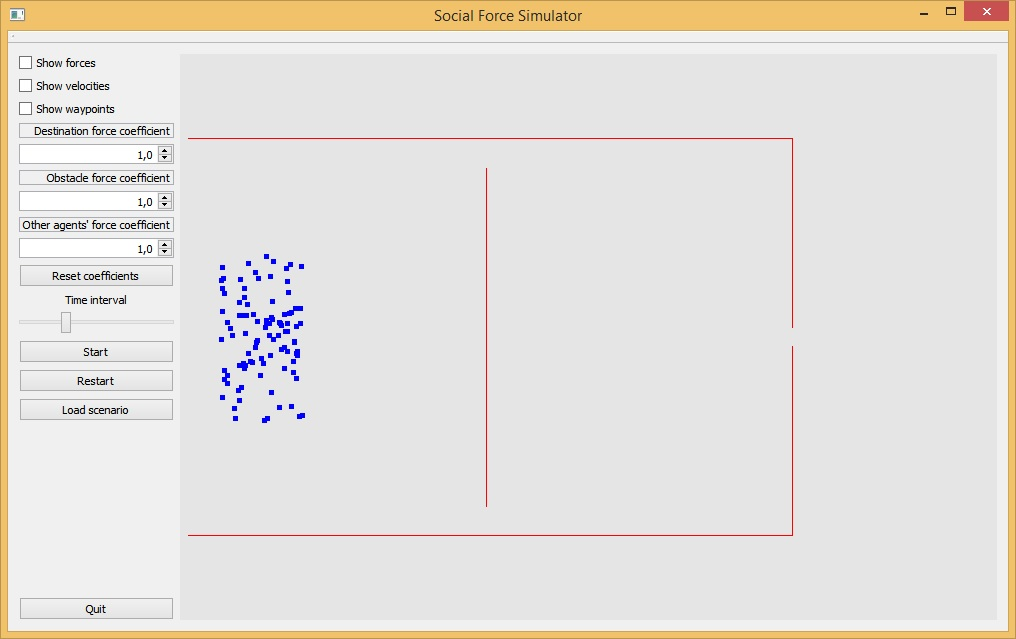
\includegraphics[scale=0.5]{ui}
\caption{Interfejs użytkownika}
\end{figure}

\subsection{Różnice implementacji w porównaniu z wersją książkową}
\hspace{4ex}Do obliczania siły interakcji pomiędzy agentem a agentami z otoczenia nie bierzemy pod uwagę wszystkich agentów ze sceny, tylko tych z najbliższego otoczenia.
Kolejną zmianą jest to, że do obliczenia sił interakcji uwzględniamy tylko najbliższą przeszkodę, a nie wszystkie znajdujące się na mapie. W wyniku symulacji zmieniliśmy też parametry siły interakcji z przeszkodami na $a=1.3$ i $b=0.8$. Symulacje na naszym modelu z książkowymi parametrami nie dawały satysfakcjonującego wyniku. Na agentów działało zbyt duże przyspieszenie, dlatego dodaliśmy do równania zmiany prędkości parametr $\alpha$
$$v_{new} = \alpha * v_{actual} + a * t $$
gdzie $\alpha = 0.5$

\subsection{Inicjalizowanie sceny}
\hspace{4ex}Jak już wcześniej wspomnieliśmy, inicjalizowanie sceny odbywa się z pliku w formacie XML.

Cały scenariusz zawiera się wewnątrz znacznika $<scenario> ... </scenario>$.

\subsubsection{Deklaracja waypoint'ów}
\hspace{4ex}Najpierw definiujemy waypoint'y, czyli punkty przez które muszą przejść agenci. Waypoint ma \emph{id}, współrzędne \emph{x} i \emph{y}, a także promień \emph{r}.

\begin{lstlisting}
  <waypoint id="1" x="-0.92" y="0" r="0.02" />
\end{lstlisting}

\subsubsection{Deklaracja agentów}
\hspace{4ex}Definowanie agenta jest trochę bardziej skomplikowane. Każdy agent posiada współrzędne \emph{x} i \emph{y} oraz liczbę generowanych agentów \emph{n} i parametry \emph{dx} i \emph{dy}. \emph{n} agentów jest generowanych ze współrzędnymi początkowymi $(x \pm dx, y \pm dy)$. Dodatkowo dla tych agentów dodaje się waypointy za pomocą znacznika $<addwaypoint ... />$ z \emph{id} waypointa, które musi się zgadzać, z którymś z waypoint'ów zadeklarowanych wcześniej. Kolejność dodawania waypoint'ów jest istotna; w takiej kolejności będą zmierzali do nich agenci. Całość definicji agenta zamykamy w znaczniku $<agent> ... </agent>$. Przykład:

\begin{lstlisting}
<agent x="-0.7" y="0" n="100" dx="0.2" dy="0.4">
    <addwaypoint id="2" />
</agent>
\end{lstlisting}

\subsubsection{Deklaracja przeszkód(ścian)}
\hspace{4ex}Ostatnim elementem jest zadeklarowanie ścian $<obstacle ... />$.
Zawiera on współrzędne \emph{x1, y1} początku ściany oraz współrzędne \emph{x2,y2} końca ściany.

\begin{lstlisting}
 <obstacle x1="-0.9" y1="-0.9" x2="-0.9" y2="-0.03" />
\end{lstlisting}




\subsubsection{Przykładowa deklaracja scenariusza}

\begin{lstlisting}
<scenario>
  <waypoint id="1" x="-0.92" y="0" r="0.02" />
  <waypoint id="2" x="0.92" y="0" r="0.02" />
  
  <agent x="-0.7" y="0" n="100" dx="0.2" dy="0.4">
    <addwaypoint id="2" />
  </agent>
  <agent x="0.7" y="0" n="100" dx="0.2" dy="0.4">
    <addwaypoint id="1" />
  </agent>
  
  <obstacle x1="-0.9" y1="-0.9" x2="-0.9" y2="-0.03" />
  <obstacle x1="-0.9" y1="0.03" x2="-0.9" y2="0.9" />
  <obstacle x1="-0.9" y1="-0.9" x2="0.9" y2="-0.9" />
  <obstacle x1="-0.9" y1="0.9" x2="0.9" y2="0.9" />
  <obstacle x1="0.9" y1="-0.9" x2="0.9" y2="-0.03" />
  <obstacle x1="0.9" y1="0.03" x2="0.9" y2="0.9" />	
</scenario>
\end{lstlisting}


\newpage
\section{Diagramy klas UML}
\hspace{4ex}
\begin{figure}[ht]
\centering
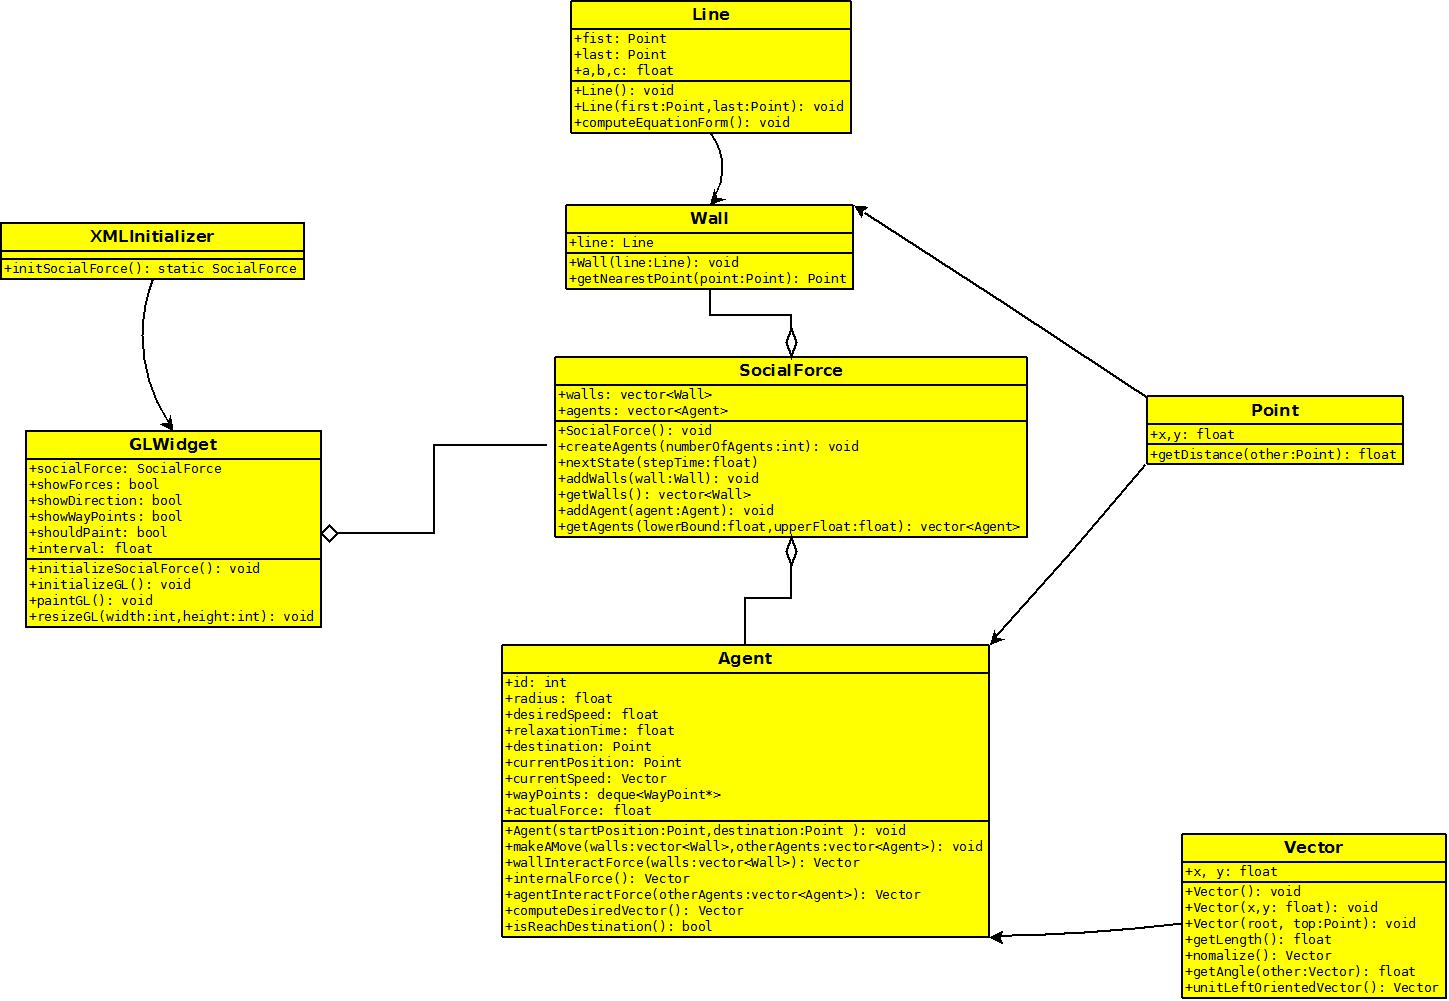
\includegraphics[scale=0.4]{ClassDiagram}
\caption{Diagram klas}
\end{figure}
\chapter{Formulacja modelu 'Social force'}
\section{Zbudowanie ogólne równanie}
\hspace{4ex}Zgodnie z koncepcją 'Social force' przez {\it Helbing \& Molnar 1995} my możemy uznać, że ruch pieszego można opisać za pomocą trzech różnych składników tak, że 
$$f_{i}^{o}$$  \centerline{wewnętrzne przyspieszenie zachowanie, odzwierciedlając motywację pieszego} \centerline{do poruszania się w określonym kierunku z określoną prędkością.} 
$$f_{i}^{wall}$$ \centerline{wpływ ścian korytarza na tego pieszego}
$$f_{ij}$$ \centerline{efekty interakcji odzwierciedlające reakcję pieszych j do innego pieszego i.}
\par \medskip W tym momencie, poznamy zmianą prędkości $v_{i}$ pieszego i coraz możemy wypisać takie równanie w formularze
$$
\frac{dv_{i}}{dt} = f_{i}^{o} + f_{i}^{wall} + f_{ij}
$$
\section{Zbudowanie komponentów}
\hspace{4ex}Łatwo widzimy, że wykorzystujemy dane eksperymentalne do sprawdzenia poprawności powyższego równania i określenia najważniejszej funkcji interakcji $f_{ij}$. Przejdźmy przez wszystkie komponenty.
\subsection{Zachowanie pojedynczego pieszego}
\hspace{4ex}Zgodnie z koncepcją 'Social force' przez {\it Helbing \& Molnar 1995} my mamy równanie dla wewnętrznego przyspieszenia zachowania $\vec{f_i^o}$:
$$\vec{f_{i}^{o}} = \frac{v_i^oe_i^o-v_{i}(t)}{\tau}$$
Gdy,\\ \centerline{$v_i^o = 1.29 \pm 0.19(ms^{-1})$ : pożądane prędkości}
\centerline{$v_i(t) (ms^{-1})$ : aktualna prękość}
\centerline{$\tau = 0.54 \pm 0.05(s)$: czas relaksacji}
\centerline{$e_i^o$: pożądany kierunek ruchu}
\subsection{Wpływ ścian na tym pieszym}
\hspace{4ex}Zgodnie z wcześniejszymi ustaleniami przez {\it Johansson et al. 2007} takie efekty ścian korytarzy na tym pieszym można opisać za pomocą równania:
$$
f_i^{wall}(d_w) = ae^{\frac{-d_w}{b}}
$$
Gdy, \\
\centerline{$d_w (m)$ : odległość prostopadła z pieszego do ściany}
\centerline{$a = 3$ i $b = 0.1$ : parametry odpowiadające do siły odpychania tego samego rzędu}
\subsection{Interakcje międzyludzkie}
\hspace{4ex}Również zgodnie z poprzednego badania poprzez {\it Johansson et al. 2007}, my też wiedzieliśmy, że interakcje międzyludzkie $f_{ij}$ mogą być definiować interakcje międzyludzkie jako funkcja odległości i kąta podejścia okazują się jasne i uzasadnione $f_{ij}(d,\theta)$ i mamy równanie dla tej funkcji
\newpage
$$
f_{ij}(d,\theta) = -Ae^{\frac{-d}{B}}(e^{-(n'B\theta)^2}t + e^{-(nB\theta)^2}n)
$$
Gdy,\\
\centerline{$d(m)$ : odległość między dwoma pieszymi $i$'em i $j$'em}
\centerline{$\theta(rad)$ : kąt między kierunkiem interakcji a wektorem skierowanym od pieszego $i$ do $j$}
\centerline{$A = 4.5 \pm 0.3$}
\centerline{$n' = 2.0 \pm 0.1$}
\centerline{$n = 3.0 \pm 0.7$}
\centerline{$t_{ij}$ : kierunek interakcji}
\centerline{$n_{ij}$ : zmiany kierunkowe}
\centerline{$B = ???????????$}

\chapter{Symulacje na komputerze}

\chapter{Podsumowanie}

\section*{Podziękowanie i referencja}

\end{document}